% THIS IS SIGPROC-SP.TEX - VERSION 3.1
% WORKS WITH V3.2SP OF ACM_PROC_ARTICLE-SP.CLS
% APRIL 2009
%
% It is an example file showing how to use the 'acm_proc_article-sp.cls' V3.2SP
% LaTeX2e document class file for Conference Proceedings submissions.
% ----------------------------------------------------------------------------------------------------------------
% This .tex file (and associated .cls V3.2SP) *DOES NOT* produce:
%       1) The Permission Statement
%       2) The Conference (location) Info information
%       3) The Copyright Line with ACM data
%       4) Page numbering
% ---------------------------------------------------------------------------------------------------------------
% It is an example which *does* use the .bib file (from which the .bbl file
% is produced).
% REMEMBER HOWEVER: After having produced the .bbl file,
% and prior to final submission,
% you need to 'insert'  your .bbl file into your source .tex file so as to provide
% ONE 'self-contained' source file.
%
% Questions regarding SIGS should be sent to
% Adrienne Griscti ---> griscti@acm.org
%
% Questions/suggestions regarding the guidelines, .tex and .cls files, etc. to
% Gerald Murray ---> murray@hq.acm.org
%
% For tracking purposes - this is V3.1SP - APRIL 2009

\documentclass{acm_proc_article-sp}

\begin{document}

\title{02333 Parallel and Real-time Systems F10}
\subtitle{[Report on the work done in this course]
\titlenote{This report is also available online at \texttt{www.notyetdecided.tld/report}}}
%
% You need the command \numberofauthors to handle the 'placement
% and alignment' of the authors beneath the title.
%
% For aesthetic reasons, we recommend 'three authors at a time'
% i.e. three 'name/affiliation blocks' be placed beneath the title.
%
% NOTE: You are NOT restricted in how many 'rows' of
% "name/affiliations" may appear. We just ask that you restrict
% the number of 'columns' to three.
%
% Because of the available 'opening page real-estate'
% we ask you to refrain from putting more than six authors
% (two rows with three columns) beneath the article title.
% More than six makes the first-page appear very cluttered indeed.
%
% Use the \alignauthor commands to handle the names
% and affiliations for an 'aesthetic maximum' of six authors.
% Add names, affiliations, addresses for
% the seventh etc. author(s) as the argument for the
% \additionalauthors command.
% These 'additional authors' will be output/set for you
% without further effort on your part as the last section in
% the body of your article BEFORE References or any Appendices.

\numberofauthors{4} %  in this sample file, there are a *total*
% of EIGHT authors. SIX appear on the 'first-page' (for formatting
% reasons) and the remaining two appear in the \additionalauthors section.
%
\author{
% You can go ahead and credit any number of authors here,
% e.g. one 'row of three' or two rows (consisting of one row of three
% and a second row of one, two or three).
%
% The command \alignauthor (no curly braces needed) should
% precede each author name, affiliation/snail-mail address and
% e-mail address. Additionally, tag each line of
% affiliation/address with \affaddr, and tag the
% e-mail address with \email.
%
% 1st. author
\alignauthor
Andreas Rask Jensen\\
%       \affaddr{}\\
%       \affaddr{}\\
       \email{s083165@student.dtu.dk}
% 2nd. author
\alignauthor
Demmus Hentze Højgaard\\
       \email{s062591@student.dtu.dk}
% 3rd. author
\alignauthor
Hjallgrim Gunnar Mohr Hentze\\
       \email{s062418@student.dtu.dk}
\and  % use '\and' if you need 'another row' of author names
% 4th. author
\alignauthor 
Kim Rostgaard Christensen\\
       \email{s084283@student.dtu.dk}
}

\maketitle
\begin{abstract}
%Abstract; A brief summary of all of the report including the conclusion section
%but excluding the acknowledgements, references and any appendixes.
The purpose of this report is to describe in detail how we implemented the tasks in the course. The overall goal is to build a tiny operating system using the technologies also available in contemporary, widely used operating systems.
\end{abstract}

% XXX Should this be here? 

% A category with the (minimum) three required fields
\category{H.4}{Information Systems Applications}{Miscellaneous}
%A category including the fourth, optional field follows...
\category{D.2.8}{Software Engineering}{Metrics}[complexity measures, performance measures]

\terms{Report}

\keywords{ACM proceedings, \LaTeX, text tagging} % NOT required for Proceedings

\section{Introduction}
\chapter{Introduction}
This report documents the design and implementation of a travel agency service The travel agency acts as a coordinator by composing and synchronizing bookings and accounts from third party actors.

\section{Introduction to Web Services}
The current trend within distributed systems is using the world wide web and it's technologies as a transportation and encapsulation layer. As these technologies are standardized, interoperability becomes less of a hassle than if every protocol should be implemented from scratch.\\\\
From the times where first static web pages emerged in the new World Wide Web, upto now, a big evolution process has taken place. This process may be described best as; chaotic. Everyone that has done web programming within the last 10 years will flee in terror by pronouncing to them the letters IE.\\
But, that aside, from this evolution it became clear that standards should drive the web forward - as they had from the days of HTTP 0.9. And as web applications grew larger and became increasingly dynamic and intercoupled, it also became clear that interfacing was a lot more problematic than what could be handled \emph{ad-hoc}.\\\\
The following section is a description of some of the key technologies we will use in this report, along with a brief discussion on some of the objective strengths and weaknesses.

\begin{description}
\item[HTTP] The \textbf{H}yper\textbf{T}ext \textbf{T}ransfer \textbf{P}rotocol is a plaintext stateless request-response protocol with standardized methods and response codes. It is deployed everywhere, from coffee machines to mainframes and thus a robust technology to base a web application on. Most programming languages have auxiliary libraries that provide both HTTP client and server components for re-use.

\item[XML] The e\textbf{X}tensible \textbf{M}arkup \textbf{L}anguage is a subset of the Standard Generalized Markup Language (SGML) and has a very famous cousin named Hypertext Markup Language - or HTML. XML is, basically, a general purpose markup language for adding semantics to documents. This semantic is further formalized by either linking a Document Type Definition (DTD), or an XML Schema (XSL) to the document. A large advantage of XML is that it, like HTTP, is a widely used standard, and most programming languages have libraries for using XML without having to parse everything. XML - being a generalized language - has the further advantage that you can build new standards as XML applications and inherit the well-formedness\footnote{Grammatically and semantically correct.} property of of XML itself, and the general XML parser can used.

\item[WSDL] \textbf{T}he \textbf{W}eb \textbf{S}ervice \textbf{D}efinition Language is an XML application introducing formalism to web application in an attempt to unify the diverging methods for collaborating via web.

\item[SOAP] \textbf{S}hoddy \textbf{O}verbloated \textbf{A}ccess \textbf{P}rotocol is another XML application % Simple Object Access Protocol
SOAP is independent of HTTP, and can therefore not inherit any information deriving from HTTP headers - even if used over HTTP.

\item[BEPL] \textbf{B}ullshit \textbf{P}olluted \textbf{E}xecution \textbf{L}anguage %Business Process Execution Language is also an XML application
%TODO Should we discuss this one, or just mention it in the bank interface section? \item[UDDI/service discovery]

\item[REST] The concept \textbf{RE}presentational \textbf{S}tate \textbf{T}ransfer covers the architecture defined by Roy Fielding and is specific application to HTTP (1.1) and centralized around the concept of resources and representations\footnote{Typically states of resources}. Resources are accessed and changed by ordinary HTTP methods: GET, PUT, POST, DELETE and standard HTTP 1.1 response codes are used to explain to the caller how the request went. For instance, a DELETE operation on a non-existing ID could return a 404 - Not Found, while it would return 200 - OK if all went well. There exists no (standardized) formalization language to describe RESTful web services, like there does with WSDL.

\item[JSON] \textbf{J}ava\textbf{S}cript \textbf{O}bject \textbf{N}otation is an object serialization language that is human-readable -- much like XML. One of the big advantages of JSON over XML is, however, that grammer, and thus effectively, the parser is very simple. It is also less verbose than XML and therefore has less overhead. It has draft support for schemas, and has currently no general way of validating data, or enforcing constraints. Due to its simple nature, it doesn't support any other types than the ones that are built-in. JSON is typically used in web applications, and in strong collaboration with the REST paradigm.

%TODO Find reference to XML book and course book.
\end{description}

\section{Related work}
%Related work; A discussion of any material not background but still related to
%the report.

\section{Body}
%Body; A number of sections describing the work done.

\subsection{Task B1 - system calls}
Task B1 is to implement a system call. This 

\subsubsection{Reflections}


\subsection{Task B2 - processes}
Task B2 was to implement process handling in out operating system. Lets look a bit closer on the concept of processes before discussing the implementation.
\subsubsection{The process concept}
A process is a in an instance of a program (an executable) that runs in an operating system environment, 
and returns to this operating system upon completion. Hence, the operating system is the one resposible for 
creating new processes and terminating them. An analogy to this is the a java object, being an instance of a java class.\\
The process is therefore nothing more than a container for resources reserved to the process by the operating system. \\

\subsubsection{The thread concept}
A thread is the part of the process container responsible for executing the program. Usually processes can have a number of threads as iliustrated in figure \ref{fig:thread_models}.(a). \\

So, the operating system need to keep track of the running processes and take care of creating and terminating the processes. 
For this, we have added two system calls; create and terminate.

\begin{figure}
\centering
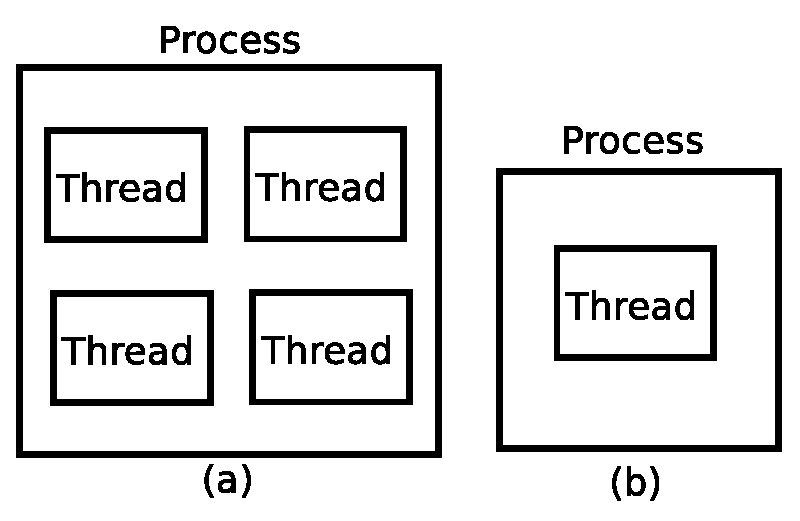
\epsfig{file=fig/Thread_Models.eps, height=1in}
\caption{Typical thread models}
\label{fig:thread_models}
\end{figure}

\subsubsection*{The create system call}
To implement this, we need to keep track of the running processes. This is handled by a process table that contains structures holding information about an individual process. \\
Processes are executed invoking this system call by executing a piece of assembler code that calls a named procedure called ``main'' and then calls terminate when main is done executing. In this system call we create one thread, and only one for each process, so our thread model actually looks like figure \ref{fig:thread_models}.(b)

\subsubsection*{The terminate system call}
When a program finishes the terminate system call is invoked. This does cleanup by of course cleaning up references to the process 
and the threads of the process, but also do a context switch. We switch back to the thread of the parent of the process just terminated.

\subsection{Reflections}

\subsubsection*{How is the system booted?}
Our virtual pc starts a BIOS that searches for a bootloader (in our case Grub), that then loads the kernel image to memory from a harddisk - or in our case a disk image. The virtual pc is an AMD64 architecture.

\subsubsection*{How are processes created from executable files?}
The kernel finds all executable files and loads them to memory, storing a pointer to the first instruction for each process. The function prepare\_process does a lot of sanity checks on the image assuring that it is in fact meant for execution.

\subsubsection*{How does a daemon (process) differ from processes studied in this task?}
Our processes runs ``interactively'' and daemons traditionally runs in the background. Otherwise they share the fact that they are started at bootup by the operating system.

\section{Test}
This task needs to have implemented the system calls ``createprocess'' and ``terminate'' so that the two executables are able to create process as stored in the executable\_table. After the executables have reached the end of their code they will make the system call to terminate. This desired result was achieved as defined in task definition, and the test was a success.

\subsection{Task B3 - scheduling}
%concepts
\subsubsection{Reflections}

\subsubsection*{question?}

\section{Conclusions}
%Conclusions; All experiences and conclusions drawn from the work.
The group widely known as group 42 would like to thank everyone for their support and free coffee.\\

\subsection{Threading}
The threading works rather well, but is very limited as it only has one thread in a process. If this was to be implemented, most of the
process handling code should be rewritten.

\subsection{Scheduling}
% ready for multithreading in processes.


%ACKNOWLEDGMENTS are optional
\section{Acknowledgments}
\input{acknowledgements.tex}
%Acknowledgments; Acknowledge any persons important to the work.

%References; A list of reference material used. All material must be cited in the
%text.



% The following two commands are all you need in the
% initial runs of your .tex file to
% produce the bibliography for the citations in your paper.
\bibliographystyle{abbrv}
\bibliography{sigproc}  % sigproc.bib is the name of the Bibliography in this case
% You must have a proper ".bib" file
%  and remember to run:
% latex bibtex latex latex
% to resolve all references
%
% ACM needs 'a single self-contained file'!
%
%APPENDICES are optional
%\balancecolumns
\appendix
%Appendix A

%Appendixes; Appendixes holds, for example, results or figures that are not
%relevant to place in the body of the report. Appendixes should generally be
%avoided and might not be read by the course staff.


\section{Code examples}

\end{document}
